\documentclass{beamer}
\usetheme{metropolis}           % Use metropolis theme
\usepackage{listings}
\usepackage{booktabs}

\lstset{language=Python}
\lstset{label={lst:code_direct}}
\lstset{basicstyle=\scriptsize, showstringspaces=false}


\title{Legal Semantic Modeling}
\date{May 5, 2020}

\author{Harout Boujakjian, Clara Buss, Elizabeth Kenis, Tim Rogers, Ahn Hoang}

\institute{George Mason University}

\begin{document}

\maketitle


\begin{frame}
  \frametitle{Background}
  \footnotesize
  \begin{itemize}
  \item Veterans submit tons of appeals each year to BVA regarding PTSD diagnosis.
  \item BVA must sift through all of these cases.
  \item Automating argument mining can be very helpful!
  \item Do legal documents have any sort of structure?
  \end{itemize}
\end{frame}

\begin{frame}
  \frametitle{BVA sample raw case}
  \centering
  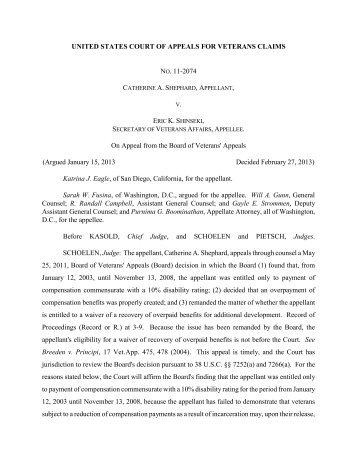
\includegraphics[width=0.6\linewidth]{BVAcase.jpg}
\end{frame}

\begin{frame}
  \frametitle{Data set}
  \begin{itemize}
  \item Data set contains 20 cases (2,526 sentences in total)
  \item Before preprocessing, the data set only has two columns (sentence, rhetorical role)
  \item Each sentence has labeled rhetorical role by LLT lab
  \item Not your typical ``Big Data'' NLP problem! Falls under multiclass classification.
    \begin{figure}
    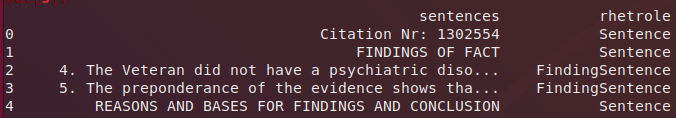
\includegraphics[width=1\linewidth]{sample_data.png}
    \end{figure}
  \end{itemize}
\end{frame}


\begin{frame}
  \frametitle{Rhetorical Roles}
  \footnotesize
  Examples
  \begin{itemize}
  \item \textbf{Finding of Fact}: The Veteran is not service-connected for any disability.
  \item \textbf{Reasoning}: He is a lay person, as there is no indication that he possesses medical knowledge, training, or experience.
  \item \textbf{Evidence}: Diagnoses of schizoaffective disorder were made in VA treatment records and at the February 2008 VA mental disorders examination.
  \item \textbf{Legal Rule}: A current disability exists when there is a disability when a claim for it is filed or at any time during the pendency of such claim.
  \item \textbf{Citation}: McClain v. Nicholson, 21 Vet. App. 319 (2007).
  \end{itemize}
\end{frame}


\begin{frame}
  \frametitle{Preprocessing}
   \footnotesize
  \begin{itemize}
  \item Remove stop words and convert all words to lower case
  \item In order to create predictors, the sentences must be tokenized into individual words.
    \item The tokens will then be transformed using Bag of Words or TD-IDF
      \item This will create the dataframe (or dataframe) of numerical values to run the models on
  \end{itemize}
\end{frame}

\begin{frame}
  \frametitle{Modeling and Metrics}
  \begin{itemize}
    \item Potential models: regularized logistic regression, neural network, random forest
      \item Confusion matrix and classification report (precision, recall, F1-score)
  \end{itemize}

  \end{frame}


\end{document}